\documentclass[usenames,dvipsnames,t]{beamer}

\usepackage[english]{babel}
\usepackage[utf8]{inputenc}
\usepackage{amsmath,amsthm, amssymb, latexsym}
\usepackage{amssymb}
\usepackage{color}
\usepackage{tikz}
\usepackage{standalone}
\usepackage{minted}
\usepackage{lmodern}
\usepackage{fontawesome}

\definecolor{DarkGray}{RGB}{5, 66, 81}
\definecolor{DarkerGray}{RGB}{3, 22, 27}

\usemintedstyle{native}

\usetikzlibrary{decorations.pathmorphing}
\usetikzlibrary{decorations.pathreplacing,angles,quotes}
\tikzset{
    ultra thick/.style={line width=3pt}
}

\usecolortheme[dark,accent=cyan]{solarized}
\beamertemplatenavigationsymbolsempty
\setbeamerfont{block title}{size=\Large}
\usepackage[orientation=portrait,size=a1,scale=1.4]{beamerposter}
\newcommand{\R}{\mathbb{R}}

%%%%%%%%%%%%%%%
\usepackage{multicol}

\makeatletter
\renewenvironment{thebibliography}[1]
     {\begin{multicols}{2}[\section*{\refname}]%
      \@mkboth{\MakeUppercase\refname}{\MakeUppercase\refname}%
      \list{\@biblabel{\@arabic\c@enumiv}}%
           {\settowidth\labelwidth{\@biblabel{#1}}%
            \leftmargin\labelwidth
            \advance\leftmargin\labelsep
            \@openbib@code
            \usecounter{enumiv}%
            \let\p@enumiv\@empty
            \renewcommand\theenumiv{\@arabic\c@enumiv}}%
      \sloppy
      \clubpenalty4000
      \@clubpenalty \clubpenalty
      \widowpenalty4000%
      \sfcode`\.\@m}
     {\def\@noitemerr
       {\@latex@warning{Empty `thebibliography' environment}}%
      \endlist\end{multicols}}
\makeatother
%%%%%%%%%%%%%%%
%%%%%%%%%%%%%%%%%%%%%%%%%%%%%%%%%%%%%%%%%%%%%%%%%%%%%%%%%%%%%%%%%%%%%%%%%%%%%%%
\begin{document}

%%%%%%%%%%%%%%%%%%%%%%%%%%%%%%%%TITLE%%%%%%%%%%%%%%%%%%%%%%%%%%%%%%%%%%%%%%%%%%%
\begin{columns}
    \begin{column}{.9\linewidth}
    \vspace{1cm}

    \centering
    \textcolor{orange}{\fontsize{100}{200} \selectfont THE POWER OF MEMORY}
    \vspace{0.5cm}

    \Large\textcolor{orange}{In interactions both social and biological is memory
    size advantageous?}
    \end{column}
    \begin{column}{.1\linewidth}
        \vspace{0.5cm}
    
            
\includegraphics[width=0.8\textwidth]{static/cardiff_uni_logo}
        \end{column}
\end{columns}
%%%%%%%%%%%%%%%%%%%%%%%%%%%%%%%%FIRST ROW%%%%%%%%%%%%%%%%%%%%%%%%%%%%%%%%%%%%%%%
\begin{columns}
    \begin{column}{.1\linewidth}
    \end{column}
    \begin{column}{.2\linewidth}
        \vspace{1.1cm}

        \begin{itemize}
            \item Both players are better of choosing Cooperation (3)
            \item there is always a temptation for a player to Defect (5).
        \end{itemize}
    \end{column}
    \begin{column}{.09\linewidth}
    \end{column}
    \begin{column}{.17\linewidth}
        \vspace{0.1cm}

        \large{
        \begin{equation}\label{eq:payoff_matrix}
             \bordermatrix{~ & C & D \cr
                              C & (3, 3) & (5, 0) \cr
                              D & (0, 5) & (1, 1) \cr}
            \end{equation}}
    \end{column}
    \begin{column}{.09\linewidth}
    \end{column}
    \begin{column}{.3\linewidth}
        \begin{center}
            \includestandalone[width=.8\textwidth, height=0.4\textwidth]{static/memory_one}
        \end{center}
    \end{column}
    \begin{column}{.1\linewidth}
    \end{column}
\end{columns}
\vspace{0.3cm}

\hrule height 5pt
%%%%%%%%%%%%%%%%%%%%%%%%%%%%%%%%%PART ONE%%%%%%%%%%%%%%%%%%%%%%%%%%%%%%%%%%%%%%%
\begin{columns}
    \begin{column}{.05\linewidth}
    \end{column}
    \begin{column}{.4\linewidth}
        \vspace{0.9cm}

        \begin{center}
        \textcolor{orange}{\large{1. OPTIMAL MEMORY ONE STRATEGY IN A MATCH}}
        \end{center}
        \vspace{0.3cm}

        \small{
        Depending on the simultaneous moves of the two players, there are four
        possibles `states':}

        \begin{center}
            \includestandalone[width=.5\textwidth]{static/states}
        \end{center}

        \small{
        A memory one strategy is denoted by the probabilities of cooperating after each of these states \(p = (p_1, p_2, p_3, p_4) \in \R_{[0,1]} ^ 4\).%~\cite{Nowak1990}.
        A match between two memory one players \(p\) and \(q\) can be modelled as
        a Markov chain.}

        \begin{equation*}
        M = \left[\begin{matrix}p_{1} q_{1} & p_{1} \left(- q_{1} + 1\right) & q_{1} \left(- p_{1} + 1\right) & \left(- p_{1} + 1\right) \left(- q_{1} + 1\right)\\
        p_{2} q_{3} & p_{2} \left(- q_{3} + 1\right) & q_{3} \left(- p_{2} + 1\right) & \left(- p_{2} + 1\right) \left(- q_{3} + 1\right)\\
        p_{3} q_{2} & p_{3} \left(- q_{2} + 1\right) & q_{2} \left(- p_{3} + 1\right) & \left(- p_{3} + 1\right) \left(- q_{2} + 1\right)\\
        p_{4} q_{4} & p_{4} \left(- q_{4} + 1\right) & q_{4} \left(- p_{4} + 1\right) & \left(- p_{4} + 1\right) \left(- q_{4} + 1\right)\end{matrix}\right]
        \end{equation*}
        \vspace{0.3cm}

        Thus the utility of player \(p\) against an opponent \(q\) is given by:

            \[u_q(p) = v \times S_{p}\]
            \vspace{0.3cm}

        where \(v\) denotes the stationary vector of \(M\) and \(S_{p}\) the payoffs of
        player \(p\) given by equation~(\ref{eq:payoff_matrix}).
        \vspace{0.5cm}

        \textcolor{solarizedGreen}{Against a single opponent:}
        \vspace{0.3cm}

        \[\max_q: u_q(p) = \frac{\frac{1}{2}\enspace p  Q  p^T + c^T p + a} 
                        {\frac{1}{2}\enspace  p  \bar{Q}  p^T + \bar{c}^T  p + \bar{a}}\]

         \[st:  \ p \in \R^4_{[0, 1]}\]
         \vspace{0.3cm}

        \small{
        where \(Q, \bar{Q}\) are matrices of \(4 \times 4\), and \(c, \bar{c}\) are 
        \(4 \times 1\) vectors  defined with the transition probabilities of the
        opponent's transition probabilities \(q_1, q_2, q_3, q_4\).}
    \vspace{2cm}

%%%%%%%%%%%%%%%%%%%%%%%%%%%%%%%%%%%PART THREE%%%%%%%%%%%%%%%%%%%%%%%%%%%%%%%%%%%
    \textcolor{orange}{\large{3. OPTIMAL MEMORY ONE IN A TOURNAMENT}}
    \vspace{0.3cm}

    \small{
        In order to find the optimal memory on player against a set of opponents
        we need to explore the numeration of the differentiation of:
        \vspace{0.3cm}

        \[\dots\]

        \vspace{0.3cm}
        \small{
        This will be explored using the \textbf{resultant}.}

    }

    \begin{center}
        \includestandalone[width=.5\textwidth]{static/resultant}
    \end{center}

    \small{
        \begin{itemize}
            \item Dixon's resultant;
            \item Maycalay resultant.
        \end{itemize}
    }
    \end{column}

%%%%%%%%%%%%%%%%%%%%%%%%%%%%%%%%%%%PART TWO%%%%%%%%%%%%%%%%%%%%%%%%%%%%%%%%%%%%%
    \begin{column}{.05\linewidth}
    \end{column}
    \begin{column}{.45\linewidth}
        \vspace{0.9cm}
    
        \textcolor{orange}{\large{2. WHAT IS THE OPTIMAL PURE RANDOM STRATEGY?}}
        \vspace{0.3cm}

        \small{
        A memory one strategy where the transition probabilities of each
        state are the same is called a \textbf{purely random strategy}.}
        \vspace{0.5cm}

        \textcolor{solarizedGreen}{Against a single opponent:}
        \vspace{0.3cm}

        \[ \max_q: u_q(p) = \frac{n_2p^2 + n_1p +n_0 } {d_1p + d_0}\]
        \vspace{0.3cm}

        \begin{equation*}
            \begin{aligned}
                st: & \ p_1 = p_2 = p_3 = p_4 = p\\
                & \ p \in \R_{[0, 1]} 
            \end{aligned}
        \end{equation*}
        \vspace{0.3cm}

        \small{
        The optimal behaviour of a \textbf{purely random} player \((p, p, p, p)\)
        against a memory one opponent \(q\) is given by:}
        
        \[p^* = \text{argmax}(u_q(p)), \ p \in S_q,\]
        \vspace{0.3cm}

        \small{
        where the set \(S_q\) is defined as,}
        
        \[S_q = \left \{0, p_{\pm}, 1 \left | \begin{array}{l} 0 < p_{\pm} < 1,
            \\ p_{\pm} \neq \frac{-d_0}{d_1} \end{array} \right. \right\}\]
        \vspace{0.5cm}
        
        \begin{center}
            \begin{figure}
            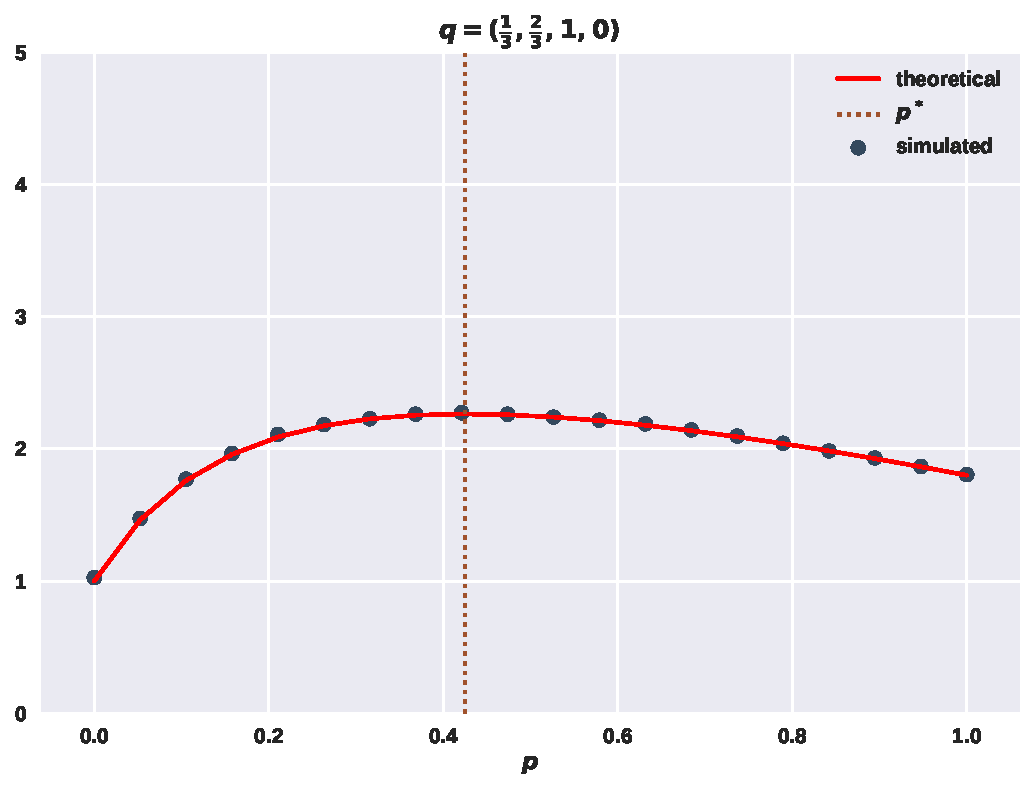
\includegraphics[width=0.6\textwidth]{static/random_vs_one}
            % \caption{The theoretical results were generated with~\cite{sympy, numpy},
            % the simulated ones with~\cite{axelrod}.}
            \end{figure}
        \end{center}
        \vspace{0.5cm}

        \textcolor{solarizedGreen}{Against multiple opponents:}
        \vspace{0.5cm}

        \[\max_q: \ \frac{\sum_{i=1} ^ {N} {u_q}^{(i)} (p)}{N}\]
        \begin{equation*}
            \begin{aligned}
            st: & \ p_1 = p_2 = p_3 = p_4 = p\\
                & \ p \in \R_{[0, 1]} 
            \end{aligned}
            \end{equation*}
            \vspace{0.3cm}

            \small{
            The optimal behaviour of a \textbf{purely random} player \((p, p, p, p)\)
            in an \(N-\)memory one player tournament, \(\{q_{(1)}, q_{(2)} \dots,q_{(N)} \}
            \) is given by:}
            \vspace{0.3cm}

            \[p^* = \text{argmax}(\displaystyle \sum_{i=1} ^ {N} {u_q}^{(i)} (p)), \ p \in S_{q(i)},\]
            \vspace{0.3cm}
            
            \small{
            where the set \(S_{q(i)}\) is defined as:}
            \vspace{0.3cm}

            \[ S_{q(i)} =  \overset{2N}{\underset{\lambda_i \neq \frac{do_i}{d1_i}}{\underset{i=1}{u}}} \lambda_i \cup \{0, 1\} \]
            \vspace{0.3cm}

            Note the size of candidate solutions is \( 1 \leq|S_{q(i)}| \leq 2N + 2\).
            \vspace{0.3cm}

            \begin{center}
                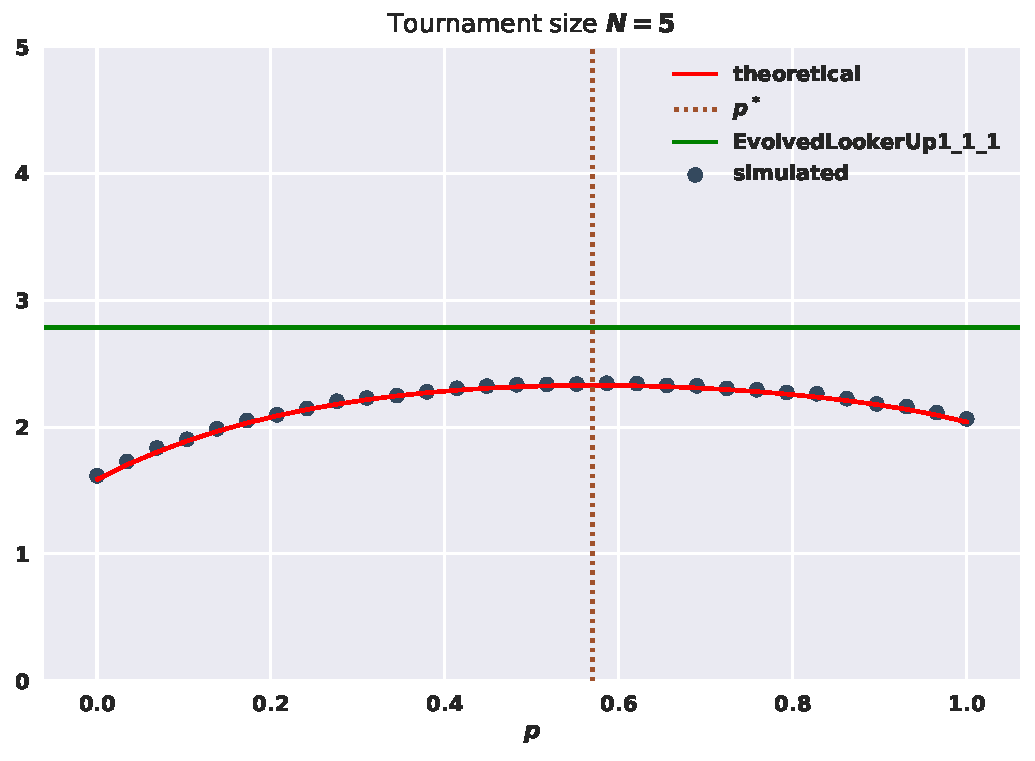
\includegraphics[width=0.6\textwidth]{static/random_vs_multiple}
            \end{center}
            \vspace{0.3cm}
    \end{column}
    \begin{column}{.05\linewidth}
    \end{column}
\end{columns}
\hrule height 5pt 
\begin{columns}
    \begin{column}{.05\linewidth}
    \end{column}
    \begin{column}{.20\linewidth}
        \vspace{0.7cm}

        \faTwitter \ NikoletaGlyn
    \end{column}
    \begin{column}{.20\linewidth}
        \vspace{0.7cm}

        \faGithub \ Nikoleta-v3}
    \end{column}
    \begin{column}{.55\linewidth}
        % \scriptsize{
        % \bibliographystyle{abbrv}
        % \bibliography{bibliography.bib}}
    \end{column}
\end{columns}
\end{document}
